\section{Extensions of linear models}


\newcommand{\datasetplot}[1]{
    \begin{tikzpicture}
        \begin{axis}[
            height=5cm,
            width=8cm,
            xmin=0,
            xmax=1,
            xtick pos=bottom,
            ytick pos=left,
            ymajorticks=false
        ]
            \ifnum#1=0
                \addplot[
                    only marks,
                    blue,
                    samples=100,
                    domain=0:1,
                    opacity=0.5
                ] (x, 20 + 5 * x + rand);
            \fi
            \ifnum#1=1
                \addplot[
                    only marks,
                    blue,
                    samples=100,
                    domain=0:1,
                    opacity=0.5
                ] (x, 20 + x^3 * 5 + rand);
            \fi
            \ifnum#1=2
                \addplot[
                    only marks,
                    blue,
                    samples=100,
                    domain=-1:1,
                    opacity=0.5
                ] coordinates {
                    (0.1, 0)
                    (0.15, 0)
                    (0.22, 0)
                    (0.4, 0)
                    (0.25, 0)
                    (0.55,0)
                    (0.43, 0)
                    (0.51, 0)
                };
                \addplot[
                    only marks,
                    blue,
                    samples=100,
                    domain=-1:1,
                    opacity=0.5
                ] coordinates {
                    (0.3, 1)
                    (0.47, 1)
                    (0.52, 1)
                    (0.65, 1)
                    (0.81, 1)
                    (0.84,1)
                    (0.91, 1)
                    (0.99, 1)
                };
            \fi
            \ifnum#1=3
                \addplot[
                    only marks,
                    blue,
                    samples=100,
                    domain=-1:1,
                    opacity=0.5
                ] coordinates {
                    (0.1, 0)
                    (0.15, 0)
                    (0.22, 0)
                    (0.4, 0)
                    (0.25, 0)
                    (0.55,0)
                    (0.43, 0)
                    (0.51, 0)
                };
                \addplot[
                    only marks,
                    blue,
                    samples=100,
                    domain=-1:1,
                    opacity=0.5
                ] coordinates {
                    (0.3, 1)
                    (0.47, 1)
                    (0.52, 1)
                    (0.65, 1)
                    (0.81, 1)
                    (0.84,1)
                    (0.91, 1)
                    (0.99, 1)
                };
                \addplot[
                    domain=0:1,
                    samples=100,
                    thick,
                    red
                ] {1 / (1 + exp(-(20 * (x - 0.5))))};
            \fi
            \ifnum#1=4
                \addplot[
                    only marks,
                    blue,
                    samples=100,
                    domain=0:1,
                    opacity=0.5
                ] (x, 20 + x^3 * 5 + rand);
                \addplot[
                    thick,
                    red,
                    samples=100,
                    domain=0:1
                ] (x, 20+x^3*5);
            \fi

            \ifnum#1=5
                \addplot[
                    only marks,
                    blue,
                    samples=100,
                    domain=0:1,
                    opacity=0.5
                ] (x, {x <= 0.2 ? 30*x + rand: (x <= 0.7 ? 6 + 10*(x-0.2) + rand: 10 + -5*(x-0.8) + rand)});
            \fi

            \ifnum#1=6
                \addplot[
                    only marks,
                    blue,
                    samples=100,
                    domain=0:1,
                    opacity=0.25
                ] (x, {x <= 0.2 ? 30*x + rand: (x <= 0.7 ? 6 + 10*(x-0.2) + rand: 10 + -5*(x-0.8) + rand)});
                \addplot[
                    very thick,
                    red,
                    domain=0:0.2
                ] (x, 20*x^0.75);

                \addplot[
                    very thick,
                    orange,
                    domain=0.2:0.6
                ] (x, 3.7+10.5*x^0.95);
                \addplot[
                    very thick,
                    yellow,
                    domain=0.6:1.0
                ] (x, 10-x^7+0.5*x^4);
            \fi

            \ifnum#1=7
                \addplot[
                    only marks,
                    blue,
                    samples=100,
                    domain=0:1,
                    opacity=0.25
                ] (x, {x <= 0.2 ? 30*x + rand: (x <= 0.7 ? 6 + 10*(x-0.2) + rand: 10 + -5*(x-0.8) + rand)});
                \addplot[
                    very thick,
                    black,
                    domain=0:1.0
                ] (x, 3.94*x^3-24.81*x^2+29.49*x+0.31);
            \fi
        \end{axis}
    \end{tikzpicture}
}

\newsavebox{\linearbox}
\sbox{\linearbox}{
    \datasetplot{0}
}

\newsavebox{\exponentialbox}
\sbox{\exponentialbox}{
    \datasetplot{1}
}

\newsavebox{\logisticbox}
\sbox{\logisticbox}{
    \datasetplot{2}
}

\newsavebox{\logregbox}
\sbox{\logregbox}{
    \datasetplot{3}
}

\newsavebox{\expregbox}
\sbox{\expregbox}{
    \datasetplot{4}
}

\newsavebox{\complexbox}
\sbox{\complexbox}{
    \datasetplot{5}
}

\newsavebox{\splinebox}
\sbox{\splinebox}{
    \datasetplot{6}
}

\newsavebox{\singlesplinebox}
\sbox{\singlesplinebox}{
    \datasetplot{7}
}

\newcommand{\gammadistribution}{
    \begin{tikzpicture}
        \begin{axis}[
            domain=0:15,
            samples=100,
            xlabel={$y$},
            width=8cm,
            height=6cm,
            xmin=0,
            xmax=15,
            ymin=0,
            ymax=0.2,
            ymajorticks=false,
            ylabel={Probability density}
        ]
        \addplot[blue, thick] {x^(2-1)*exp(-x/2)/(2^2*gamma(2))};
        \end{axis}
    \end{tikzpicture}
}

\begin{frame}{Non-linear models: Nothing to worry about}
    \begin{tikzpicture}
        \RInputNode{(0, 1.5)}{rnode}{10cm}{8}{
            formula <- ...^^J
            result <- glm(formula, family=Gamma(link="log"), data=data)^^J
        }

        \RInputNode{(0, 0)}{rnode}{10cm}{8}{
            formula <- ...^^J
            result <- gam(formula, data=data)^^J
        }
        \PythonInputNode{2}{(0, -1.5)}{glmnode}{10cm}{8}{
            from xgboost import XGBClassifier^^J
            ^^J
            model = XGBClassifier()^^J
            model.fit(X, y)^^J
        }
    \end{tikzpicture}
\end{frame}

\begin{frame}{Extensions of linear models: Generalized linear models}
    \begin{tikzpicture}
        \node[] at (-5.25, -3.5) {};
        \node[] at (5.25, 3.5) {};

        \visible<1-3,5>{
            \node[] at (0, -2.5) {
                $\hat{y}=$$\beta_0+\sum\limits_{i=0}^p \beta_ix_i$
            };
        }

        \visible<2>{
            \node[] at (0, 1) {
                \usebox{\linearbox}
            };
        }
        \visible<3-4,12>{
            \node[] at (0, 1) {
                \usebox{\exponentialbox}
            };
        }
        \visible<4>{
            \node[] at (0, -2.5) {
                $\hat{y}=$\textcolor{red}{$\beta_0+\sum\limits_{i=0}^p \beta_ix_i$}
            };
        }
        \visible<5-7>{
            \node[] at (0, 1) {
                \usebox{\logisticbox}
            };
        }
        \visible<6>{
            \node[] at (0, -2.5) {
                $\log\left(\dfrac{p(X)}{1 - p(X)}\right)=\beta_0+\sum\limits_{i=0}^p \beta_ix_i$
            };
        }
        \visible<7-8>{
            \node[] at (0, -2.5) {
                $p(X)=\dfrac{e^{\left(\beta_0+\sum\limits_{i=0}^p \beta_ix_i\right)}}{1 + e^{\left(\beta_0+\sum\limits_{i=0}^p \beta_ix_i\right)}}$
            };
        }
        \visible<8-11>{
            \node[] at (0, 1) {
                \usebox{\logregbox}
            };
        }
        \visible<9>{
            \node[] at (0, -2.5) {
                $p(X)=\dfrac{e^{\left({\color{red}\beta_0+\sum\limits_{i=0}^p \beta_ix_i} \right)}}{1 + e^{\left({\color{red}\beta_0+\sum\limits_{i=0}^p \beta_ix_i}\right)}}$
            };
        }
        \visible<10>{
            \node[] at (0, -2.5) {
                $p(X)=f(\beta_0+\sum\limits_{i=0}^p \beta_ix_i)$
            };
        }
        \visible<11-12>{
            \node[] at (0, -2.5) {
                $f(\hat{y})=\beta_0+\sum\limits_{i=0}^p \beta_ix_i$
            };
        }
        \visible<13>{
            \node[] at (0, 1) {
                \usebox{\expregbox}
            };
            \node[] at (0, -2.5) {
                $\log(\hat{y})=\beta_0+\sum\limits_{i=0}^p \beta_ix_i$
            };
        }
        \visible<14>{
            \node[] at (0, 0) {
                \gammadistribution
            };
        }
        \visible<15>{
            \node[align=flush left, text width=10.1cm] at (0, 0) {
                \textbf{Generalized linear models (GLMs):}\\
                Extends upon the regular linear model by associating the predictors to the response via a non-linear link function $f$.
                \begin{itemize}
                    \item Requires us to specify $f$ (often determined by investigating the distribution of the response).
                \end{itemize}
            };
        }
        \visible<16>{
            \PythonInputNode{1}{(-4.25, 3)}{gammanode}{9.1cm}{8}{
                from sklearn.linear_model import GammaRegressor^^J
                ^^J
                model = GammaRegressor()^^J
                model.fit(X, y)^^J
            }

            \PythonInputNode{2}{($ (gammanode.south west) - (0, 0.2) $)}{glmnode}{9.1cm}{8}{
                import statsmodels.api as sm^^J
                ^^J
                link = sm.genmod.families.links.Log()^^J
                model = sm.GLM(y, X, family=sm.families.Gamma(link=link))^^J
                model.fit()
            }

            \RInputNode{($ (glmnode.south west) - (0, 0.7) $)}{rnode}{9.1cm}{8}{
                formula <- ...^^J
                result <- glm(formula, family=Gamma(link="log"), data=data)^^J
            }
        }
    \end{tikzpicture}
\end{frame}

\begin{frame}{Extensions of linear models: Generalized additive models}
    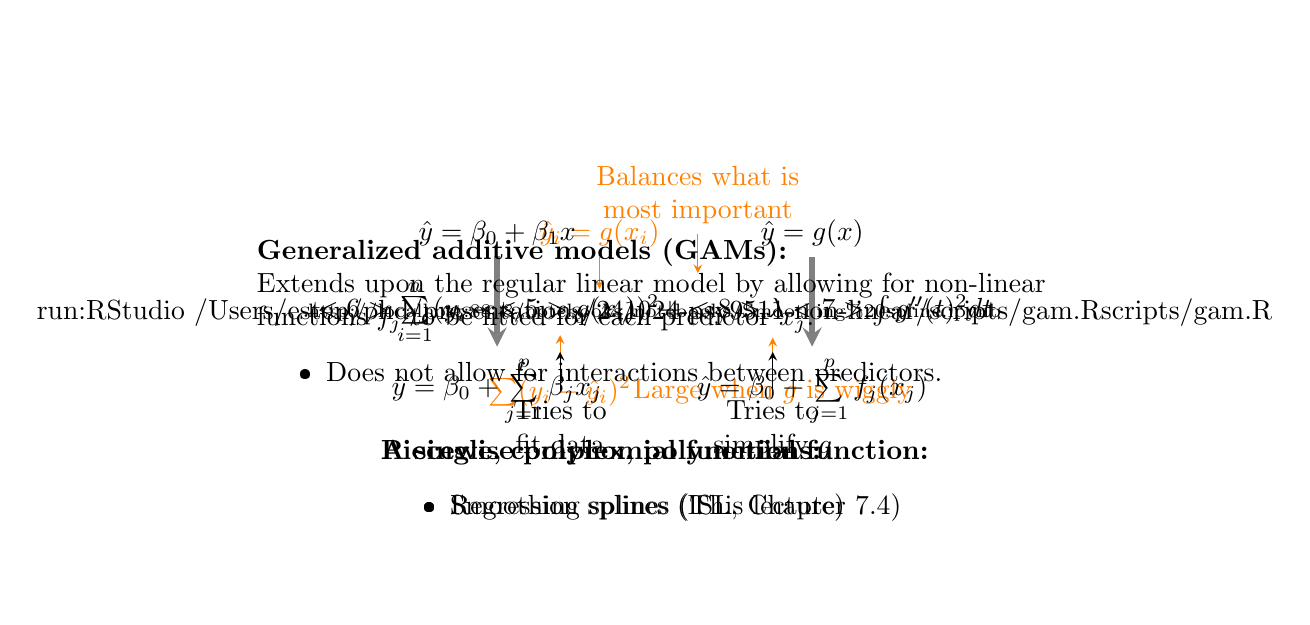
\begin{tikzpicture}
        \node[] at (-5.25, -3.5) {};
        \node[] at (5.25, 3.5) {};

        \visible<1>{
            \node[] at (0, 1) {
                \usebox{\complexbox}
            };
        }

        \visible<2>{
            \node[] at (0, 1) {
                \usebox{\splinebox}
            };
        }
         \visible<3>{
            \node[] at (0, 1) {
                \usebox{\singlesplinebox}
            };
        }


        \visible<2>{
            \node[anchor=north west, text width=10cm] at (-3.6, -1.5) {
                \textbf{Piecewise polynomial functions:}
                \begin{itemize}
                    \item Regression splines (ISL, Chapter 7.4)
                \end{itemize}
            };
        }
        \visible<3>{
            \node[anchor=north west, text width=10cm] at (-3.6, -1.5) {
                \textbf{A single, complex, polynomial function:}
                \begin{itemize}
                    \item Smoothing splines (This lecture)
                \end{itemize}
            };
        }

        \visible<4-8>{
            \node[] at (0, 0) {
                $\alert<6>{\sum\limits_{i=1}^n(y_i - \alert<5>{g(x_i)})^2} + \alert<8>{\lambda}\alert<7>{\int g''(t)^2dt}$
            };
        }

        \visible<5>{
            \node[text=orange] (model) at (-0.7, 1) {
                $\hat{y}_i=g(x_i)$
            };
            \draw[orange, -stealth] (model.south) -- +(0, -0.4);
        }
        \visible<6>{
            \node[text=orange] (mse) at (-1.2, -1) {
                $\sum (y_i - \hat{y}_i)^2$
            };
            \draw[orange, -stealth] (mse.north) -- +(0, 0.4);
        }
        \visible<7>{
            \node[text=orange] (penalty) at (1.5, -1) {
                Large when $g$ is wiggly
            };
            \draw[orange, -stealth] (penalty.north) -- +(0, 0.4);
        }
        \visible<8>{
            \node[align=center, anchor=north] (mse) at (-1.2, -1) {
                Tries to\\fit data
            };
            \draw[-stealth] (mse.north) -- +(0, 0.5);

            \node[align=center, anchor=north] (penalty) at (1.5, -1) {
                Tries to \\
                simplify $g$
            };
            \draw[-stealth] (penalty.north) -- +(0, 0.5);

            \node[align=center, anchor=south, text=orange] (lambda) at (0.55, 1) {
                Balances what is\\
                most important
            };
            \draw[-stealth, orange] (lambda.south) -- +(0, -0.5);
        }
        \only<9>{
            \node[] at (0, 0) {
                \fontsize{7}{8}\selectfont{\url{http://localhost:8888/notebooks/notebooks/Smoothing\%20spline.ipynb}}
            };
        }
        \visible<10-11>{
            \node[] (singlelinear) at (-2, 1) {
                $\hat{y}=\beta_0+\beta_1x$
            };
            \node[] (singleadditive) at (2, 1) {
                $\hat{y}=g(x)$
            };
        }
        \visible<11>{
            \node[] (multiplelinear) at (-2, -1) {
                $\hat{y}=\beta_0+\sum\limits_{j=1}^p \beta_jx_{j}$
            };
            \draw[line width=2pt, -stealth, gray] (singlelinear) -- (multiplelinear);
            \node[] (multipleadditive) at (2, -1) {
                $\hat{y}=\beta_0+\sum\limits_{j=1}^p f_j(x_{j})$
            };
            \draw[line width=2pt, -stealth, gray] (singleadditive) -- (multipleadditive);
        }
        \visible<12>{
            \node[align=flush left, text width=10.1cm] at (0, 0) {
                \textbf{Generalized additive models (GAMs):}\\
                Extends upon the regular linear model by allowing for non-linear functions $f_j$ to be fitted for each predictor $x_j$.
                \begin{itemize}
                    \item Does not allow for interactions between predictors.
                \end{itemize}
            };
        }
        \visible<13>{
            \node[] at (0, 0) {
                \href{run:RStudio /Users/esten/phd/presentations/241024-psy9511-non-linear/scripts/gam.R}{scripts/gam.R}
            };
        }

    \end{tikzpicture}
\end{frame}
